% start: template for headers and footer info that need to be adde in each pade that includes a section
\chead{\textit{IT-University of Copenhagen} \rangle  SSEQ-E2013  \rangle \textbf{Group:} 10 Danish Travel card  \rangle \textbf{ID:} 61 \rangle Responsible: All}
\cfoot{\textbf{Hand-in date:} \today \rangle \textbf{Supervisor:} Marco Nardello \rangle \textbf{Version:} 1 \rangle \textbf{Status: } Done \thepage}
\renewcommand{\headrulewidth}{0.1pt}
\renewcommand{\footrulewidth}{0.1pt}
% ends: headers/footers template

\section*{Use Case Description}

\subsection*{Actors}

\textbf{Customer:}
%A person who uses the Rejsekort system or buys it on behalf of another person.
Costumers is all kind of persons that does use \textit{Rejsekort} system to travel from a location to another, this include regular travelers, such people that goes and back from work, kinds/young that goes to school, disables, retired people. So technically an user is all costumers that uses the system.


\textbf{Customer service:}
%A person who works for the Rejsekort company serving the customers. A person in the customer service can do the same as the customer except for checking in and checking status.
Technically this a person who works for the Rejsekort's company as part of their customers service stuff. This person does have all the rights and permission to control all users account such, balance check, history, block card. But it can not control the actions that require physical response from the user such \textit{Check in} and \textit{Check out} since this only can be done by the user true a rejsekort machine or smart phone application. 


\textbf{Controller:}
%A person who checks whether passengers with Rejsekort are commuting a valid trip. In case they are not, the controller is able to issue them a fine.
The controller is the person who checks if a passenger is traveling with a properly validated card or proper checking with the mobile application. Otherwise the controller has the power to issue a fine to the infractor.


\textbf{Financial institution:}
%Withdraws money from the customers account whenever they checkout or add credit to their balance, either by them self or through the customer service.
Financial institutions can process the request from users to add credit to their rejsekort from either a credit card, Dankort or direct transfer, but this function can be trigger as well true costumer service.


\subsection*{Use cases}
% they ask for smaller font here, but if we do that, it will not be the same all over since it is just bold text, 
% so it makes no sence to follow that review.
\textbf{BlockAccount:}
An account can be blocked either by the customer or the customer service.

\textbf{CheckBalance:}
%The balance of a customer can be checked both by the customer and the customer service.
This function in the software is to allow users to check their own account balance or either call costumer service and check it true them.

\textbf{BlockCardAccount:}
A customer or the customer service can block a specific card on a customer account.

\textbf{CreateAccount:}
A customer can create an account or request the customer service to create it.

\textbf{AddBalance extends Withdraw :}
%The customer service or the customer can add balance to his account.
User can add credit to its balance or contact consumer service to do it.

\textbf{CheckOut extends Withdraw:}
When a passenger ends his commute he is able to checkout, which also can be done by the customer service in case it is needed

\textbf{Withdraw:}
%Depending of customer's choice, the financial institution withdraws money from the customers bank account when balance is added to the Rejsekort account or when checking out.
Depending of customer's choice, the financial institution withdraws money from the customers bank account, credit card or Dankort, then the balance is added to the Rejsekort account credit, also this function can be trigger if auto fill up is enable; this means the balance will auto fill up with a pre conditioned amount if the balance is too low after a commute has be done.

\textbf{CheckHistory:}
The customer service or the customer himself can check the history of activities on the account.

\textbf{CheckCustomerStatus:}
It is possible for the customer, the customer service and the controller to check whether the passenger traveling on Rejsekort have been checked in.

\textbf{SendMail:}
%Both the customer and service can communicate by mail.
Basic email communication format via email from users to costumer service and vice versa.

\textbf{EraseFine:}
The customer service can erase a fine given to a customer.

\textbf{CheckIn:}
%A passenger traveling with Rejsekort can check-in when he starts his commute and if he wish he can add:
Costumers traveling can check in, also they also have more options while check in, such as:
\begin{enumerate}
	\item AddBicycle
	\item AddAnimal
	\item AddAdult
	\item AddKid
\end{enumerate}

\textbf{GiveFine:}
The controller can give a passenger a fine.


\begin{figure}[ht!]
\centering
\makebox[\textwidth]{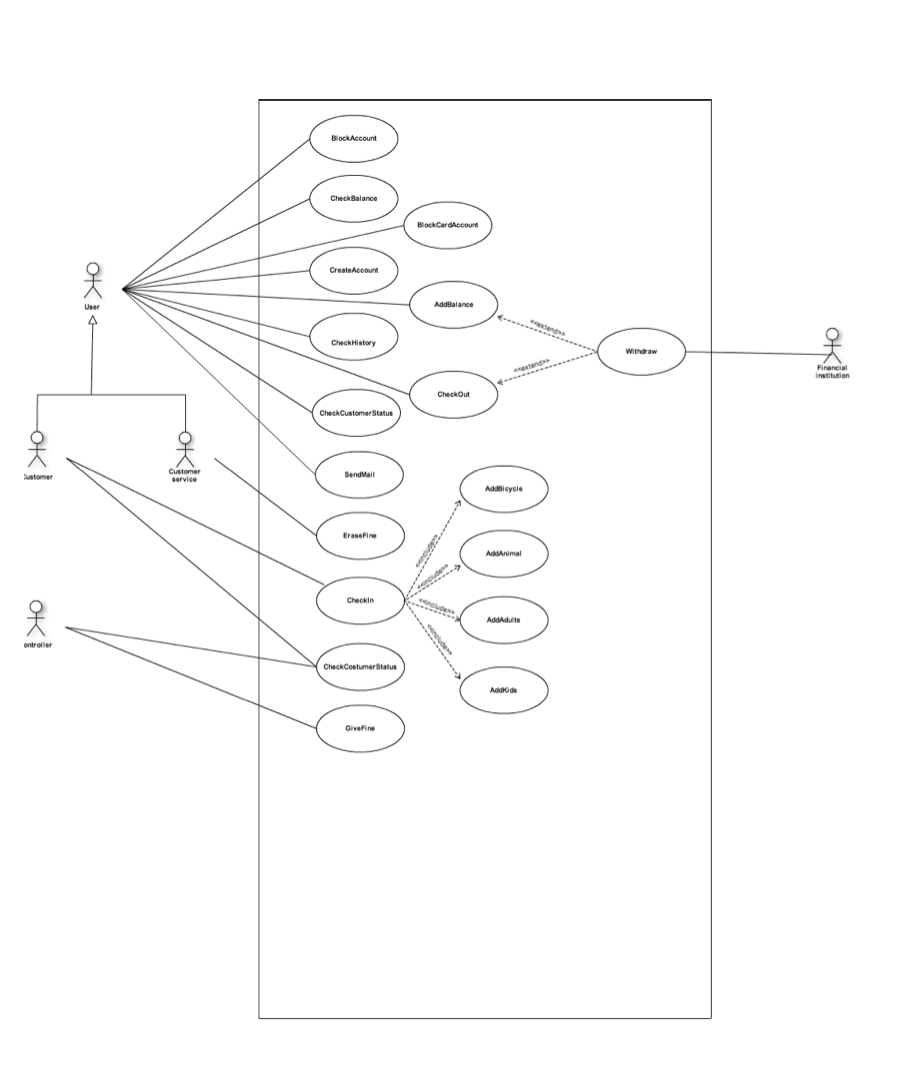
\includegraphics[width=\paperwidth]{graphics/Use_Case_Diagram.png}}
%\caption{Class Diagram}
\label{aser}
\end{figure}
